\def\retinafocusresults{
    Một đặc điểm của mô hình RetinaFocus là có nhiều cấu hình có thể cài đặt để triển khai mô hình như cấu hình lựa chọn feature maps của FPN cho nhánh Focus, cấu hình scale ảnh trong quá trình predict \dots
    Vì vậy, ta cần so sánh và lựa chọn cấu hình tối ưu nhất, cân đối giữa thời gian thực hiện quá trình predict và độ chính xác của mô hình.
    Để so sánh một cách toàn diện nhất, ta sẽ sử dụng cả hai bộ dữ liệu WIDER FACE thông thường và bộ dữ liệu WIDER FACE 4K đã được giới thiệu ở \textbf{\textit{phần 5.2}}.

    \noindent
    \textbf{\textit{Thí nghiệm so sánh cấu hình sử dụng feature maps khác nhau của FPN làm đầu vào cho nhánh Focus}} \\
    Trong thí nghiệm này, với mỗi cấu hình, chúng tôi sử dụng các feature maps khác nháu của FPN làm đầu vào cho nhánh Focus.
    Trong đó, lần lượt các cấu hình sử dụng feature maps ${C}_{3}, {C}_{4}, {C}_{5}, {P}_{3}, {P}_{4}, {P}_{5}$ được ký hiệu là \textit{C3}, \textit{C4}, \textit{C5}, \textit{P3}, \textit{P4}, \textit{P5} trong các biểu đồ.
    Trong các cấu hình trên, các cặp feature maps ${C}_{3}$ và ${P}_{3}$, ${C}_{4}$ và ${P}_{4}$, ${C}_{5}$ và ${P}_{5}$ là các cặp feature maps có cùng kích thước.
    Tuy nhiên, mỗi feature maps khác nhau trong cặp chứa thông tin khác nhau về khuôn mặt dẫn đến số lượng và kích thước của các vùng mà nhánh Focus xác định cần phải zoom vào cũng khác nhau.
    Từ đó dẫn đến thời gian thực hiện toàn bộ quá trình predict trên cả bộ dữ liệu là khác nhau.
    Trong thí nghiệm này, các cấu hình sử dụng chung một cấu hình scale ảnh trong quá trình predict là ....

    \begin{figure}[H]
        \centering
        \subfigure[]{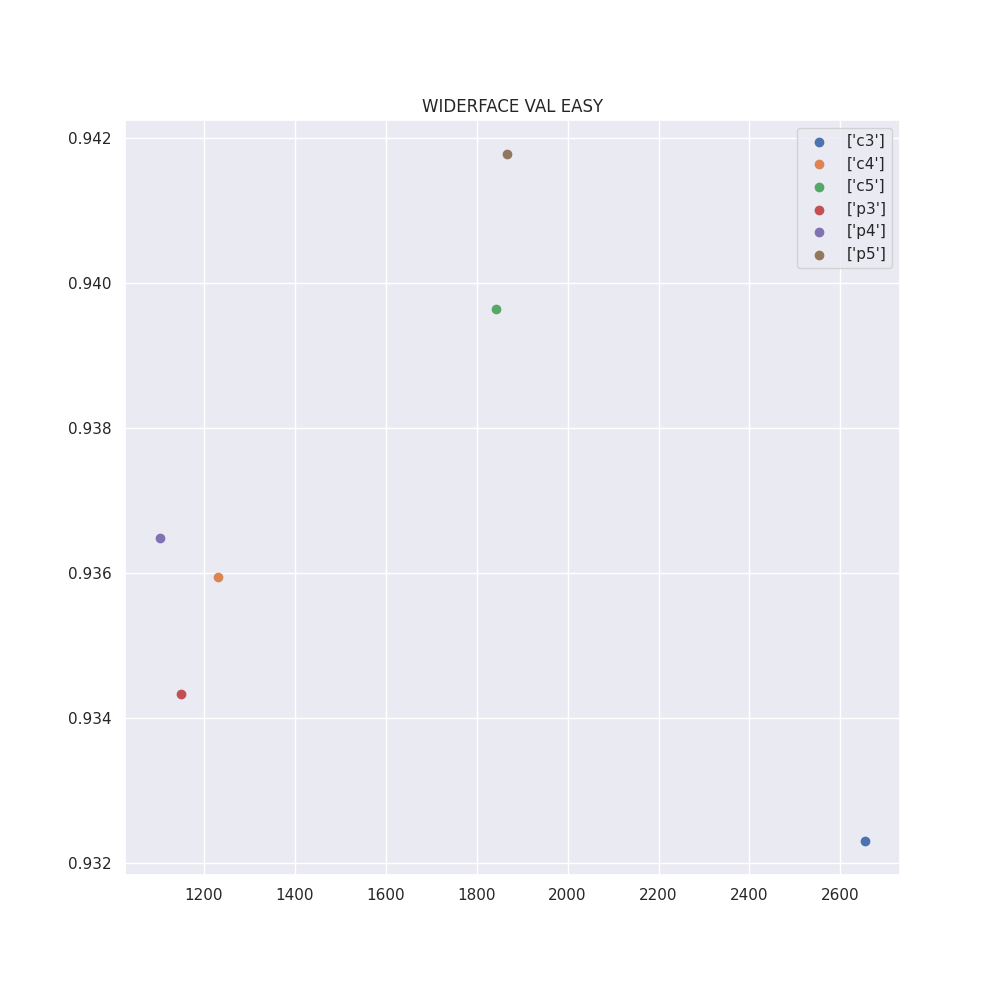
\includegraphics[width=0.32\textwidth, trim={2.3cm 2.3cm 2.3cm 2.3cm}, clip]{images/retinafocus_widerface_val_easy_fpn}} 
        \subfigure[]{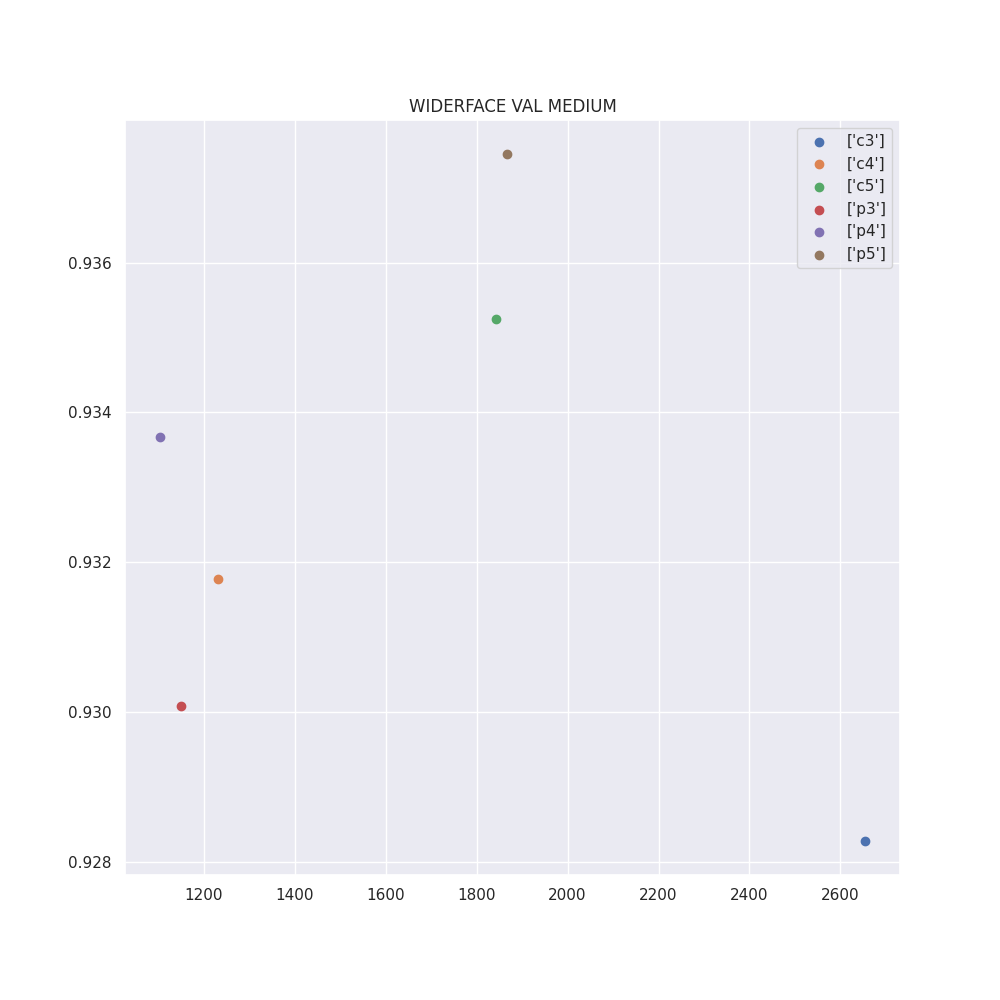
\includegraphics[width=0.32\textwidth, trim={2.3cm 2.3cm 2.3cm 2.3cm}, clip]{images/retinafocus_widerface_val_medium_fpn}} 
        \subfigure[]{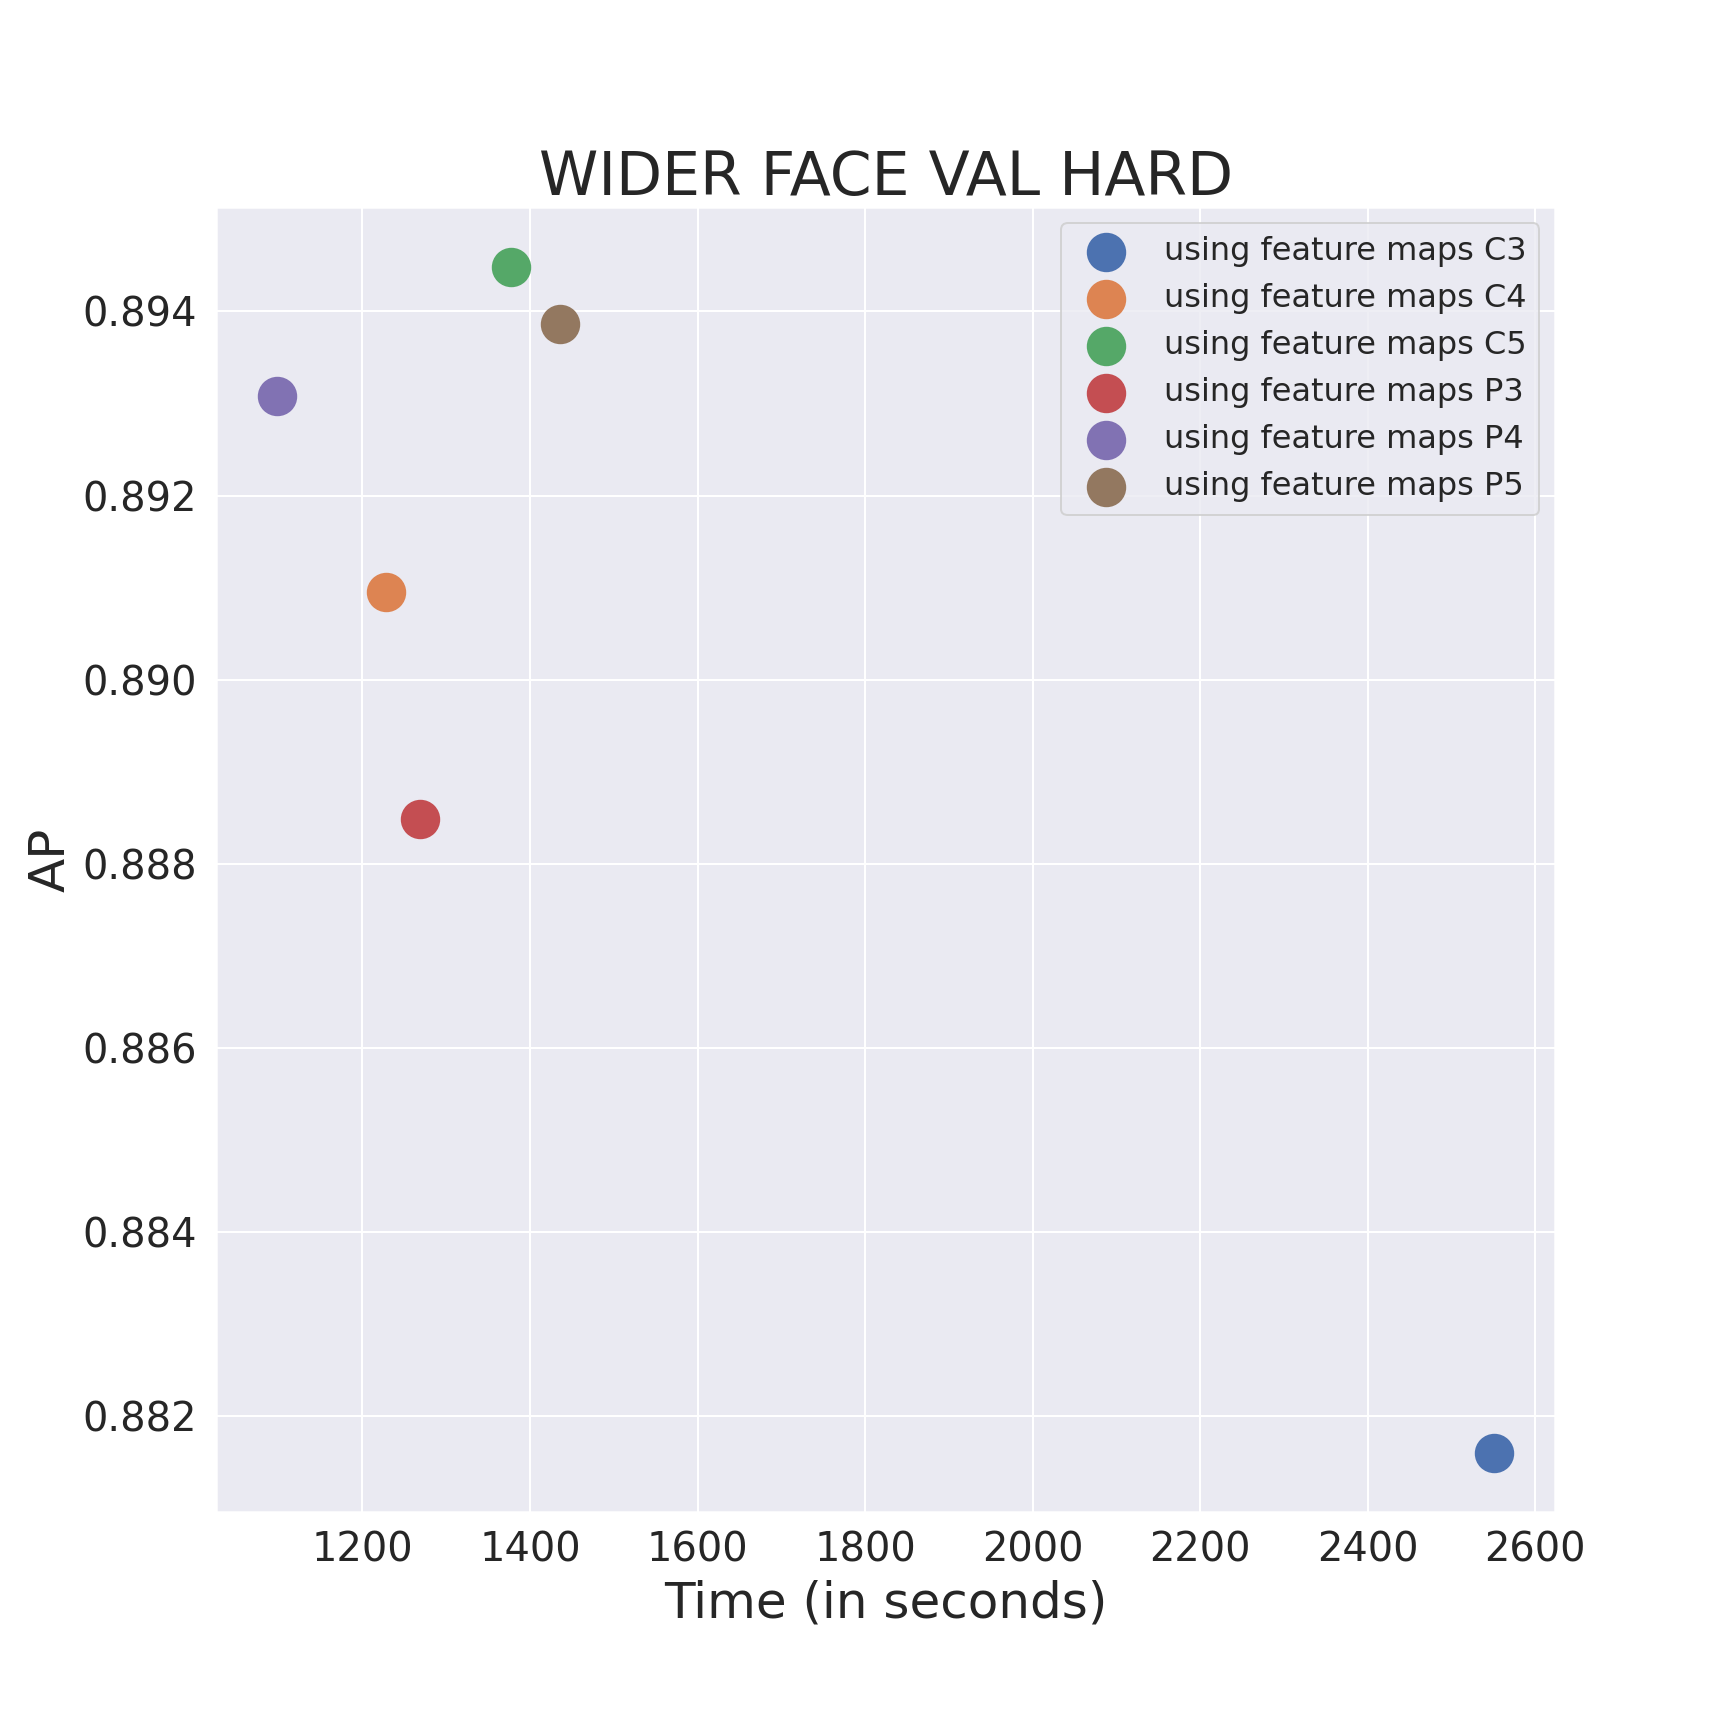
\includegraphics[width=0.32\textwidth, trim={2.3cm 2.3cm 2.3cm 2.3cm}, clip]{images/retinafocus_widerface_val_hard_fpn}} 
        \caption{Kết quả so sánh các cấu hình sử dụng các feature maps của FPN làm đầu vào cho nhánh Focus trên ba bộ dữ liệu WIDER FACE val easy (a), medium (b) và hard (c)}
        \label{fig:retinafocus_widerface_val_fpn}
    \end{figure}

    \noindent
    Đối với bộ WIDER FACE thông thường, hai cấu hình đạt độ chính xác cao nhất là cấu hình sử dụng feature maps ${P}_{5}$ và cấu hình sử dụng feature maps ${C}_{5}$ cho nhánh Focus với thời gian thực hiện toàn bộ quá trình predict trên cả bộ dữ liệu lần lượt là ... và ....
    Trong khi cấu hình sử dụng feature maps ${P}_{5}$ cho kết quả tốt hơn trên bộ WIDER FACE val easy và medium thì cấu hình sử dụng feature maps ${C}_{5}$ cho kết quả tốt hơn trên bộ WIDER FACE val hard.
    Các cấu hình khác như ${P}_{4}$, ${P}_{3}$ và ${C}_{4}$ có thời gian thực hiện toàn bộ quá trình predict nhanh hơn nhưng độ chính xác không tốt.
    Đặc biệt là cấu hình ${C}_{3}$ vừa có thời gian thực hiện toàn bộ quá trình predict chậm vừa đạt độ chính xác thấp.

    \begin{figure}[H]
        \centering
        \subfigure[]{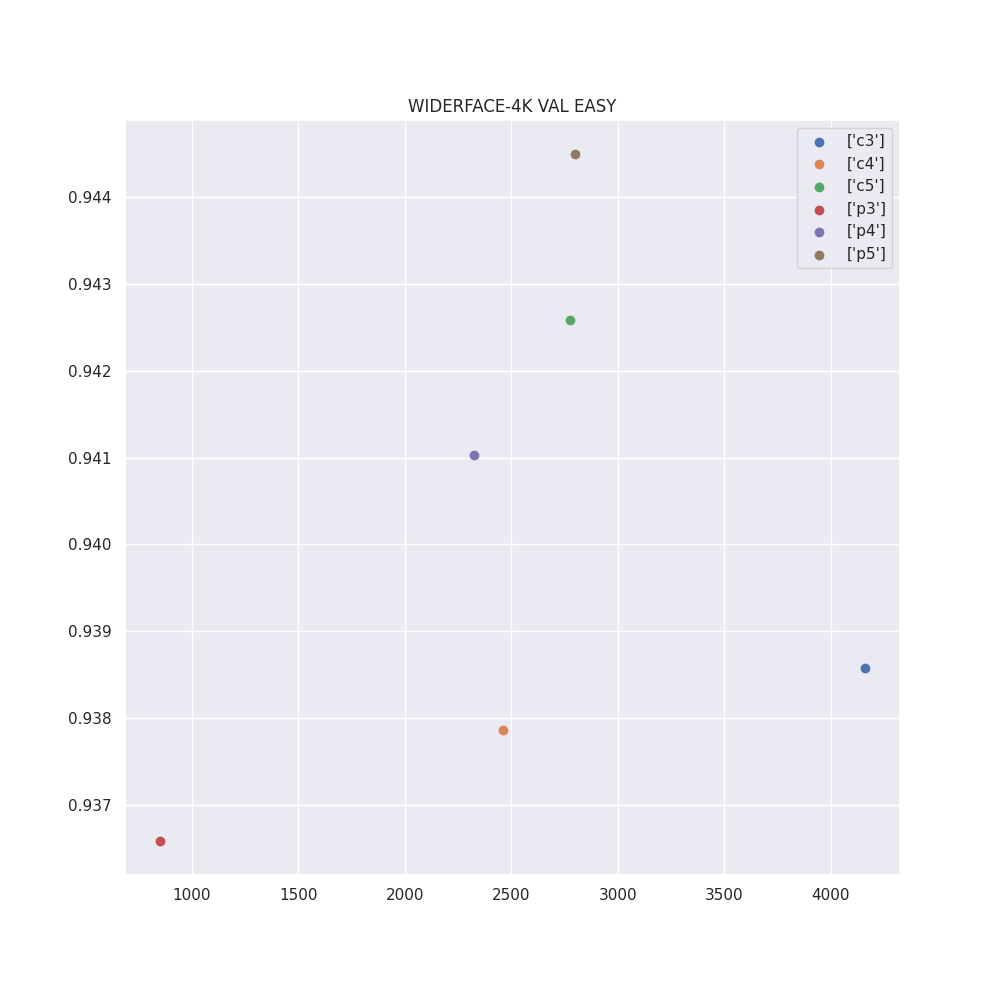
\includegraphics[width=0.32\textwidth, trim={2.3cm 2.3cm 2.3cm 2.3cm}, clip]{images/retinafocus_widerface_4k_val_easy_fpn}} 
        \subfigure[]{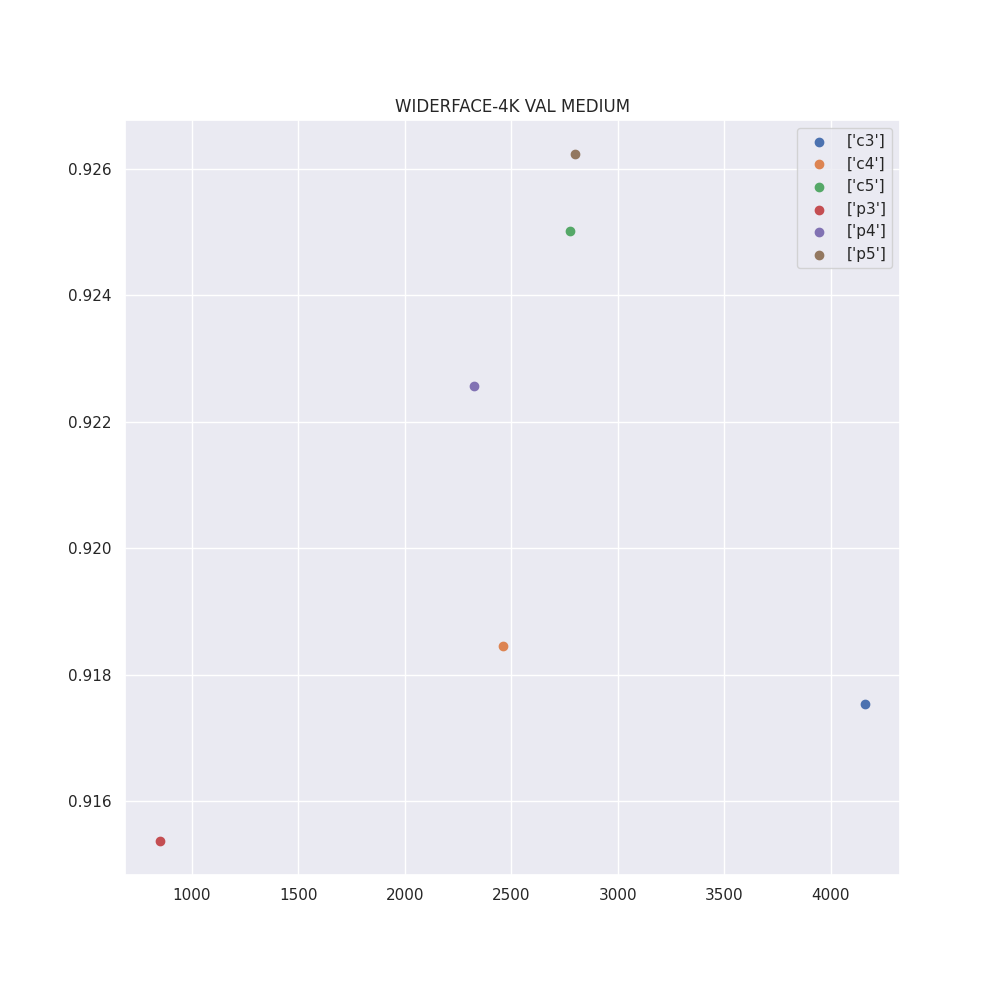
\includegraphics[width=0.32\textwidth, trim={2.3cm 2.3cm 2.3cm 2.3cm}, clip]{images/retinafocus_widerface_4k_val_medium_fpn}} 
        \subfigure[]{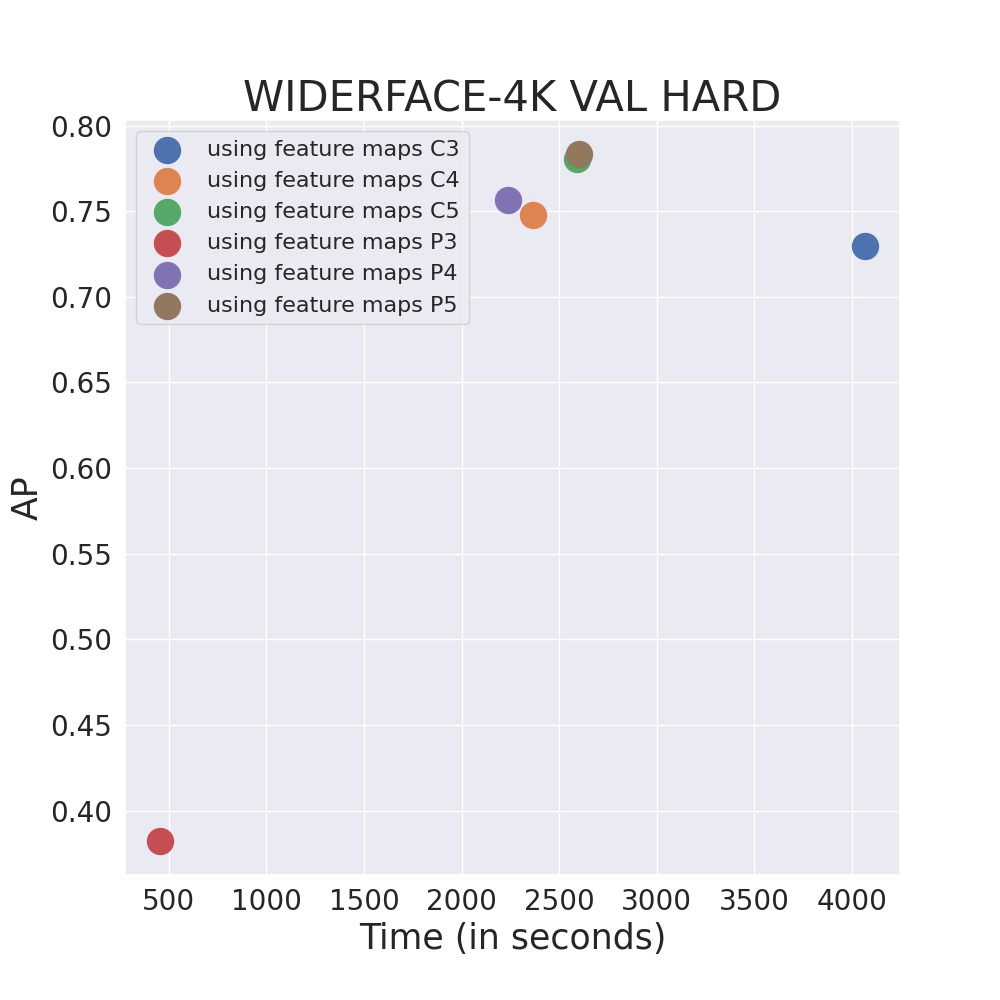
\includegraphics[width=0.32\textwidth, trim={2.3cm 2.3cm 2.3cm 2.3cm}, clip]{images/retinafocus_widerface_4k_val_hard_fpn}} 
        \caption{Kết quả so sánh các cấu hình sử dụng các feature maps của FPN làm đầu vào cho nhánh Focus trên ba bộ dữ liệu WIDER FACE 4K val easy (a), medium (b) và hard (c)}
        \label{fig:retinafocus_widerface_4k_val_fpn}
    \end{figure}

    \noindent
    Đối với bộ WIDER FACE 4K, hai cấu hình đạt độ chính xác cao nhất vẫn là cấu hình sử dụng feature maps ${P}_{5}$ và cấu hình sử dụng feature maps ${C}_{5}$ với thời gian thực hiện toàn bộ quá trình predict trên cả bộ dữ liệu lần lượt là ... và ....
    Đối với bộ dữ liệu này, cấu hình sử dụng feature maps ${P}_{5}$ cho kết quả tốt hơn so với cấu hình sử dụng feature maps ${C}_{5}$ trên cả ba bộ WIDER FACE 4K val easy, medium và hard.

    \noindent
    Kết luận đối với thí nghiệm này là cấu hình sử dụng feature maps ${P}_{5}$ đạt kết quả tốt nhất về độ chính xác trong khi vẫn duy trì được thời gian thực hiện toàn bộ quá trình predict tương đối nhanh.

    \noindent
    \textbf{\textit{Thí nghiệm so sánh cấu hình scale ảnh tốt nhất trong quá trình predict}} \\

    \noindent
    \textbf{\textit{Thí nghiệm so sánh cấu hình tốt nhất của RetinaFocus với các cấu hình của RetinaFace}} \\
    
}